\section{Running Example}
\label{sec:example}

%\begin{figure*}
%\begin{center}
%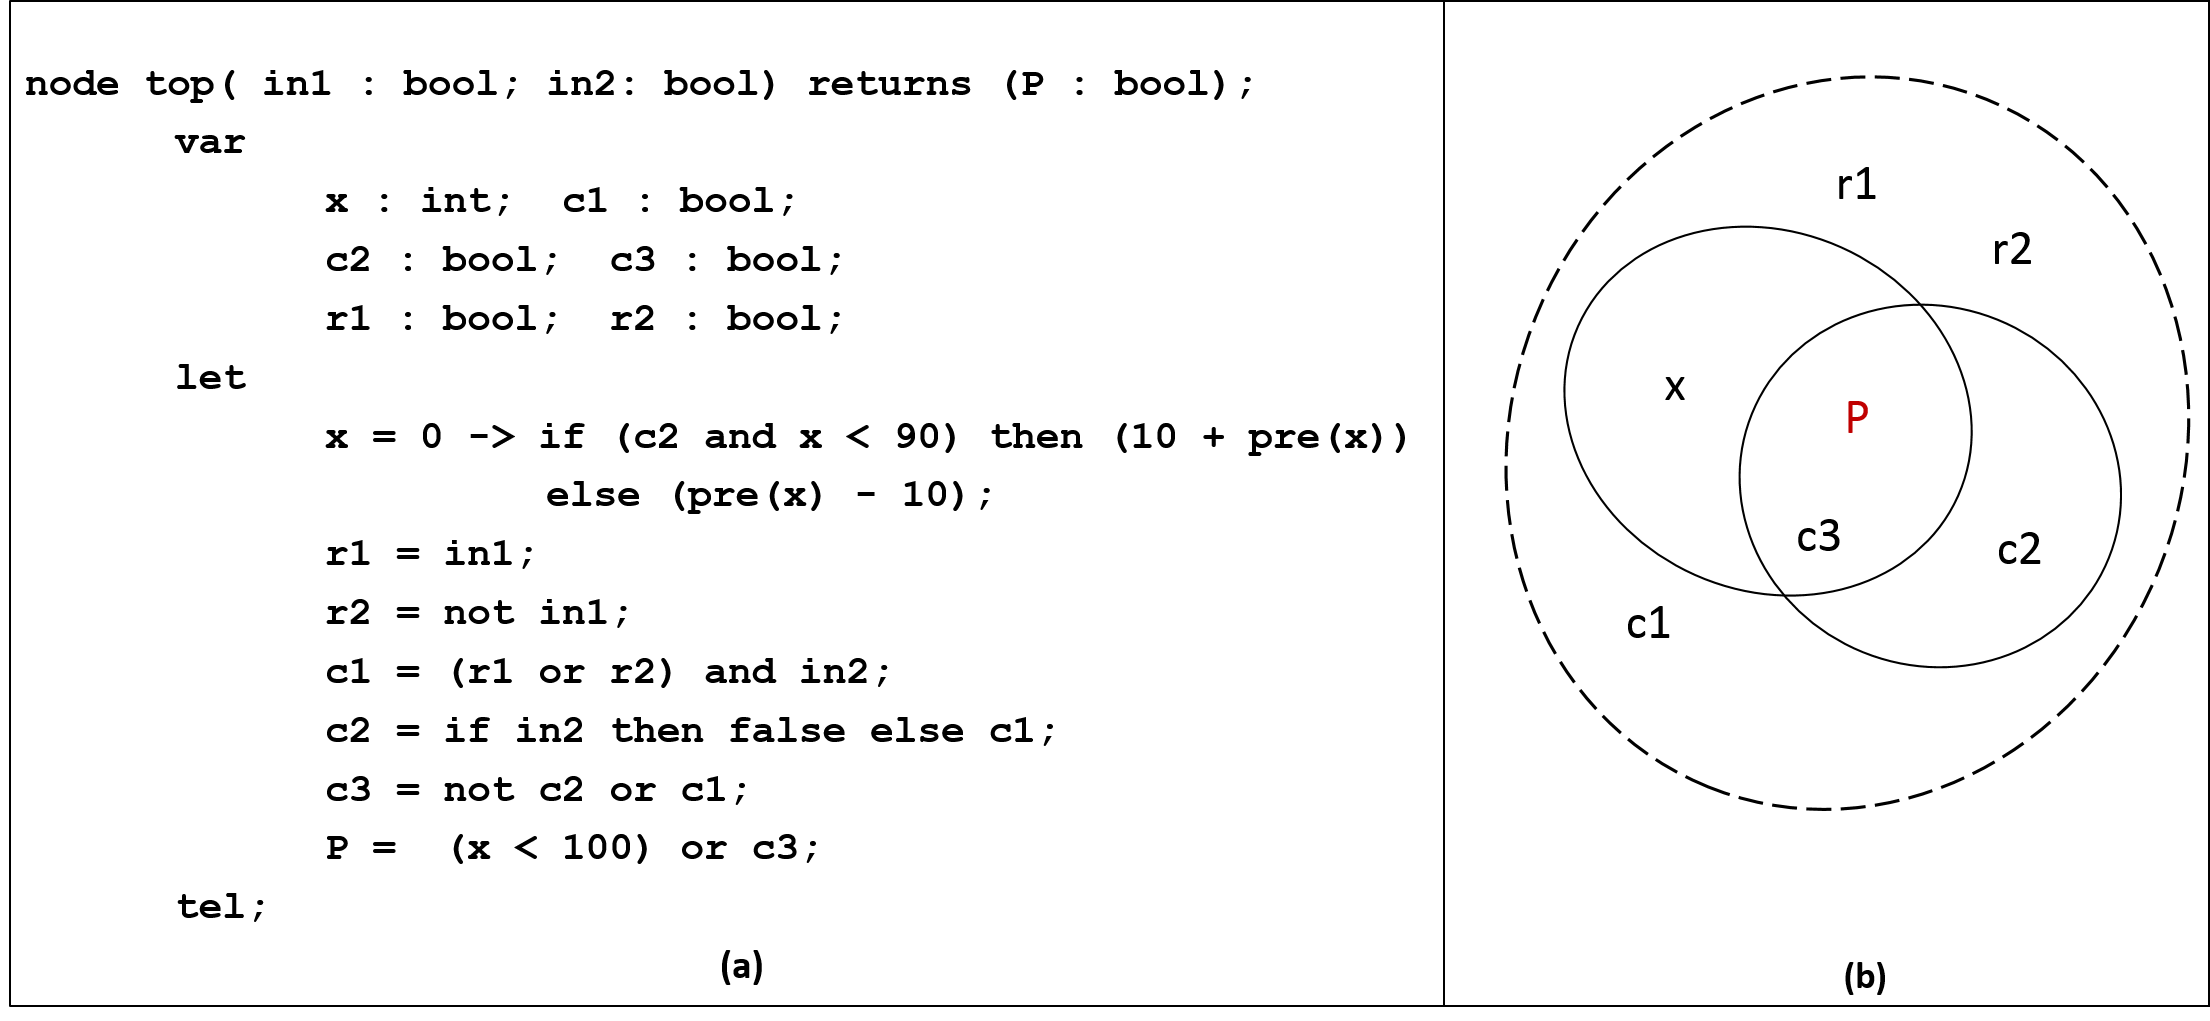
\includegraphics[width=0.8\textwidth]{figs/ex.png}
%\vspace{-0.1in}
%\caption{A Lustre model with property $P$}
%\label{fig:ex}
%\end{center}
%\end{figure*}

%% We put the image here so it shows up side-by-side with fig:ex-after
\begin{figure}[t]
\centering
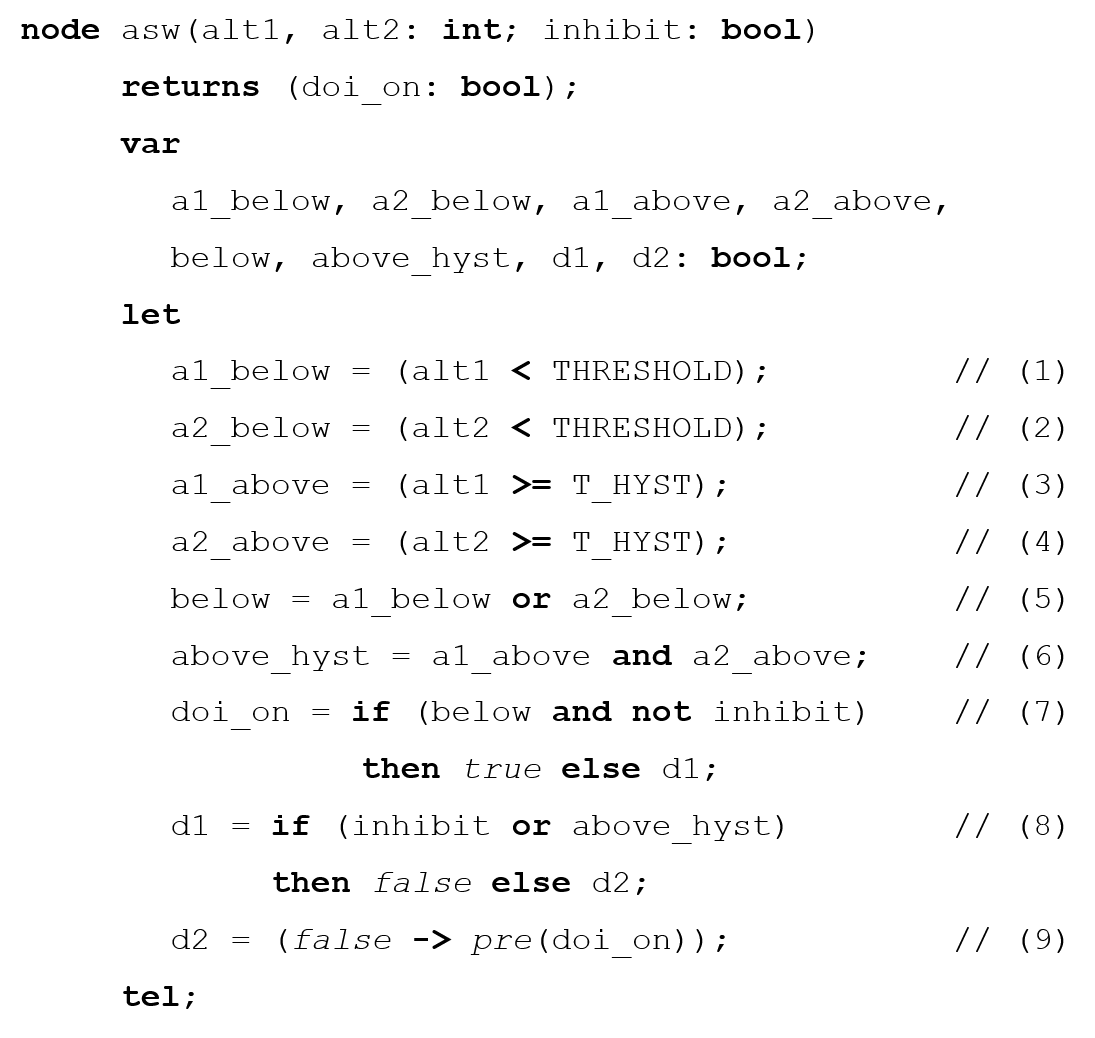
\includegraphics[width=\columnwidth]{figs/code.png}
%{\smaller
%\begin{verbatim}
%node asw(alt1, alt2: int; inhibit: bool)
%        returns (doi_on: bool);
%var
%   a1_below, a2_below, a1_above, a2_above,
%   below, above_hyst, d1, d2: bool;
%let
%   a1_below = (alt1 < THRESHOLD);        // (1)
%   a2_below = (alt2 < THRESHOLD);        // (2)
%   a1_above = (alt1 >= T_HYST);          // (3)
%   a2_above = (alt2 >= T_HYST);          // (4)
%   below = a1_below or a2_below;         // (5)
%   above_hyst = a1_above and a2_above;   // (6)
%   doi_on = if (below and not inhibit)   // (7)
%        then true else d1;
%   d1 = if (inhibit or above_hyst)       // (8)
%         then false else d2;
%   d2 = (false -> pre(doi_on));          // (9)
%tel;
%\end{verbatim}
%}
\vspace{-0.1in}
\caption{Altitude Switch Model}
\label{fig:asw}
\end{figure}

We will use a very simple system from the avionics domain to illustrate our approach. An Altitude Switch (ASW) is a hypothetical device that turns power on to another subsystem, the Device of Interest (DOI), when the aircraft descends below a threshold altitude and turns the power off again after we ascend over the threshold plus some hysteresis factor.  An implementation of an ASW containing two altimeters written in the Lustre language (simplified and adapted from~\cite{HCW02:ase-deviation}) is shown in Figure~\ref{fig:asw}.  If the system is not ``inhibited'' by the user and either altimeter is below the constant THRESHOLD, then it turns on the DOI; else, if the system is inhibited or both altimeters are above the threshold plus the hysteresis factor (THRESHOLD + HYST), then the DOI is turned off, and if neither condition holds, then in the initial computation it is false and thereafter retains its previous value.  The notation \texttt{(false -> pre(doi\_on))} in equation (9) describes an initialized register in Lustre: in the initial state, the expression is \texttt{false}, and thereafter it is the previous value of \texttt{doi\_on}.  In the remainder of the paper, we will use this model to illustrate aspects of requirements completeness.  %Section \ref{sec:illust}.


\iffalse
\mike{replace with altitude switch example!}

We will use the model in Figure~\ref{fig:ex} (a) as
a running example throughout the paper. This model is written in Lustre~\cite{Halbwachs91:lustre}, which is a synchronous dataflow language used as an input language for various model checkers. For our purposes, a Lustre program
consists of 1) input variables, {\tt in1} and {\tt in2} in the example, 2) output
variables, {\tt P} in the example, and 3) an
equation for each output variable. A Lustre program runs over discrete
time steps. On each step, the input variables take on some values and
are used to compute values for the output variables on the same step.
In addition, equations may refer to the previous value of a variable
using the {\tt pre} operator, like {\tt x} in the example. This operator is underspecified in the
first step, so the arrow operator, {\tt ->}, is used to guard the
{\tt pre} operator. In the first step the expression {\tt e1 -> e2}
evaluates to {\tt e1}, and it evaluates to {\tt e2} in all other steps. We interpret a Lustre program as a model specification by considering
the behavior of the program under all possible input traces. Safety
properties over Lustre can then be expressed as Boolean expressions in
Lustre. A safety property holds if the corresponding expression is
always true for all input traces. For example, the property for
Figure~\ref{fig:ex} is {\tt P}, which is a valid property.

In the example, the structure of the model allows property {\tt P} to be proved in two ways.
Note that {\tt c1}, {\tt r1}, and {\tt r2} do not affect the validity of {\tt P}, which means
if we remove these equations making {\tt c1}, {\tt r1}, and {\tt r2} input, still {\tt P} will be valid.
In other words, no matter what value these equations have, any change in their value is not observable in the value of {\tt P}.
However, we always need equation {\tt c3} to prove {\tt P}. In addition to {\tt c3}, in order for {\tt P} to be valid either {\tt c2} or {\tt x} is required.

In the rest of the paper, we will refer to this example while explaining different coverage notions.
\fi

%% \begin{itemize}
%%     \item Not sure if this should go before or after the background section with a description of Lustre.
%%     \item Need a small but interesting example.  Andrew, do any of the models that you use as jkind tests
%%         function in this way?  It would be nice to look at what we have lying around; we need something
%%         that requires invariants.
%%     \item It would also be good to have a few points of interest with the model-requirement pairing:
%%     \item \quad   vacuity due to an overconstrained environment
%%     \item \quad   definitions within the model that are irrelevant to the proof.
%%     \item Explain the model and the proof process.
%% \end{itemize}

%%  LocalWords:  IVC
